\subsection{GAN Mel-Spectrogram}
Using the improved Wasserstein GANs framework, we trained generators to
construct 64x64 mel-spectrogram images from a noise vector. Visual results are demonstrated below in Figure~\ref{fig:samples_comparison}.   We saw recognizable Mel-Spectrogram-like features in the
data after only 1000 generator iterations, and after 5000 iterations the generated samples were indistinguishable from real ones. Training took around 10
hours for 20000 iterations on a single 4 GB Nvidia GK104GL GPU.
%
\begin{figure}[!t]
    \centering
    \begin{subfigure}[t]{0.3\columnwidth}
        \centering
        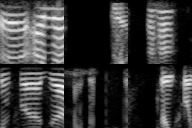
\includegraphics[width=\columnwidth]{figures/samples_groundtruth.png}
        \caption{Real (actual)}
        \label{fig:samples_real}
    \end{subfigure}
    \qquad
    \begin{subfigure}[t]{0.3\columnwidth}
        \centering
        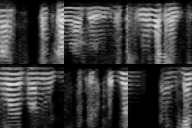
\includegraphics[width=\columnwidth]{figures/samples_5419.png}
        \caption{Fake (generated)}
        \label{fig:samples_fake}
    \end{subfigure}
    \caption{Comparison of 6 real and fake mel-spectrogram samples from all speakers. ($\sim$ 5000 generator iterations) }
    \label{fig:samples_comparison}
\end{figure}

\subsection{GAN Adversarial attacks}

Within the GAN framework, we train models for untargeted attacks by using all
data available from speakers that the speaker recognition systems was trained
on, irrespective of class label. We show in subsection \ref{sub:untargeted} that
an untargeted model able to generate data from the real distribution with enough
variety can be used to perform adversarial attacks.
Figure~\ref{fig:conf_mat_untargeted} depicts that our GAN-trained generator
successfully learns all speakers across the dataset, without mode collapsing.

As we described earlier, the models for targeted attacks can be trained in two
manners: 1) conditioning the model on additional information, e.g. class labels,
as described in~\cite{mirza2014conditional}; 2) using only data from the label
of interest. While the first approach might result in mode collapse, a drawback
of the second approach is that the discriminator, and by consequence the
generator, does not have access to universal\footnote{We draw a parallel with
Universal Background Models in speech.} properties of speech. In the targeted
attacks subsection \ref{sub:targeted} we show results using our new objective
function described in equation~\ref{eq:wgan_gp_mixed} that allows using data
from all speakers.  

\subsubsection{Untargeted attacks}\label{sub:untargeted}
For each speaker audio data in the test set, we compute a Mel-Spectrogram as
descibred in section \ref{sub:processdata}. The resulting Mel-Spectrogram is
then fed into the CNN recognizer and we extract a 1024-dimensional feature $\Phi$ from
the first fully-connected layer (L5) in the pre-trained CNN model
(\ref{fig:CNN}) trained on the real speech dataset with all speaker IDs. This
deep feature/embedding $\Phi$ is then used to train a K-nearest-neighbor (KNN)
classifier, with K equal to 5.

To control the generator trained by our WGAN-GP, we feed the generated
Mel-Spectrograms into the same CNN-L7 pipeline to extract their corresponding
feature $\widehat \Phi$. Utilizing the pre-trained KNN, each sample is assigned to
the nearest speaker in the deep feature space. Therefore, we know which speaker
our generated sample belongs to when we attack our CNN recognizer. We evaluate our
controlled WGAN-GP samples against our CNN speaker recognition system, and the
confusion matrix can be found in Figure \ref{fig:conf_mat_untargeted}. 

\subsubsection{Targeted attacks}\label{sub:targeted}
We trained the WGAN-GP on the entirety of the NIST 2004 corpus (100 speakers), a single speaker (P280) from
the VCTK Corpus, and the single speaker from the Blizzard dataset. The samples
from the other models were either downloaded from the
web or created from WaveNet globally conditioned on the single VCTK corpus
speaker, and on SampleRNN trained only on data from the Blizzard dataset.
Results for the WGAN-GP are demonstrated in Figure \ref{fig:confusion_matrices}.  
In the samples generated with sampleRNN and WaveNet models, \textbf{none} of the
predictions made by the classifier match the target speaker. 

We also trained the WGAN-GP with and without the \textbf{mixed loss} on
different speakers. The histogram of predictions in Figure
~\ref{fig:pred_comp_spk0} shows WGAN-GP results for speaker 0. The improved
WGAN-GP loss achieves 0.38 error rate and our mixed loss achieves 0.12 error
rate, producing a 75\% increase in accuracy. 

\begin{figure}[!t]
    \centering
    \begin{subfigure}[b]{0.4\columnwidth}
        \centering
        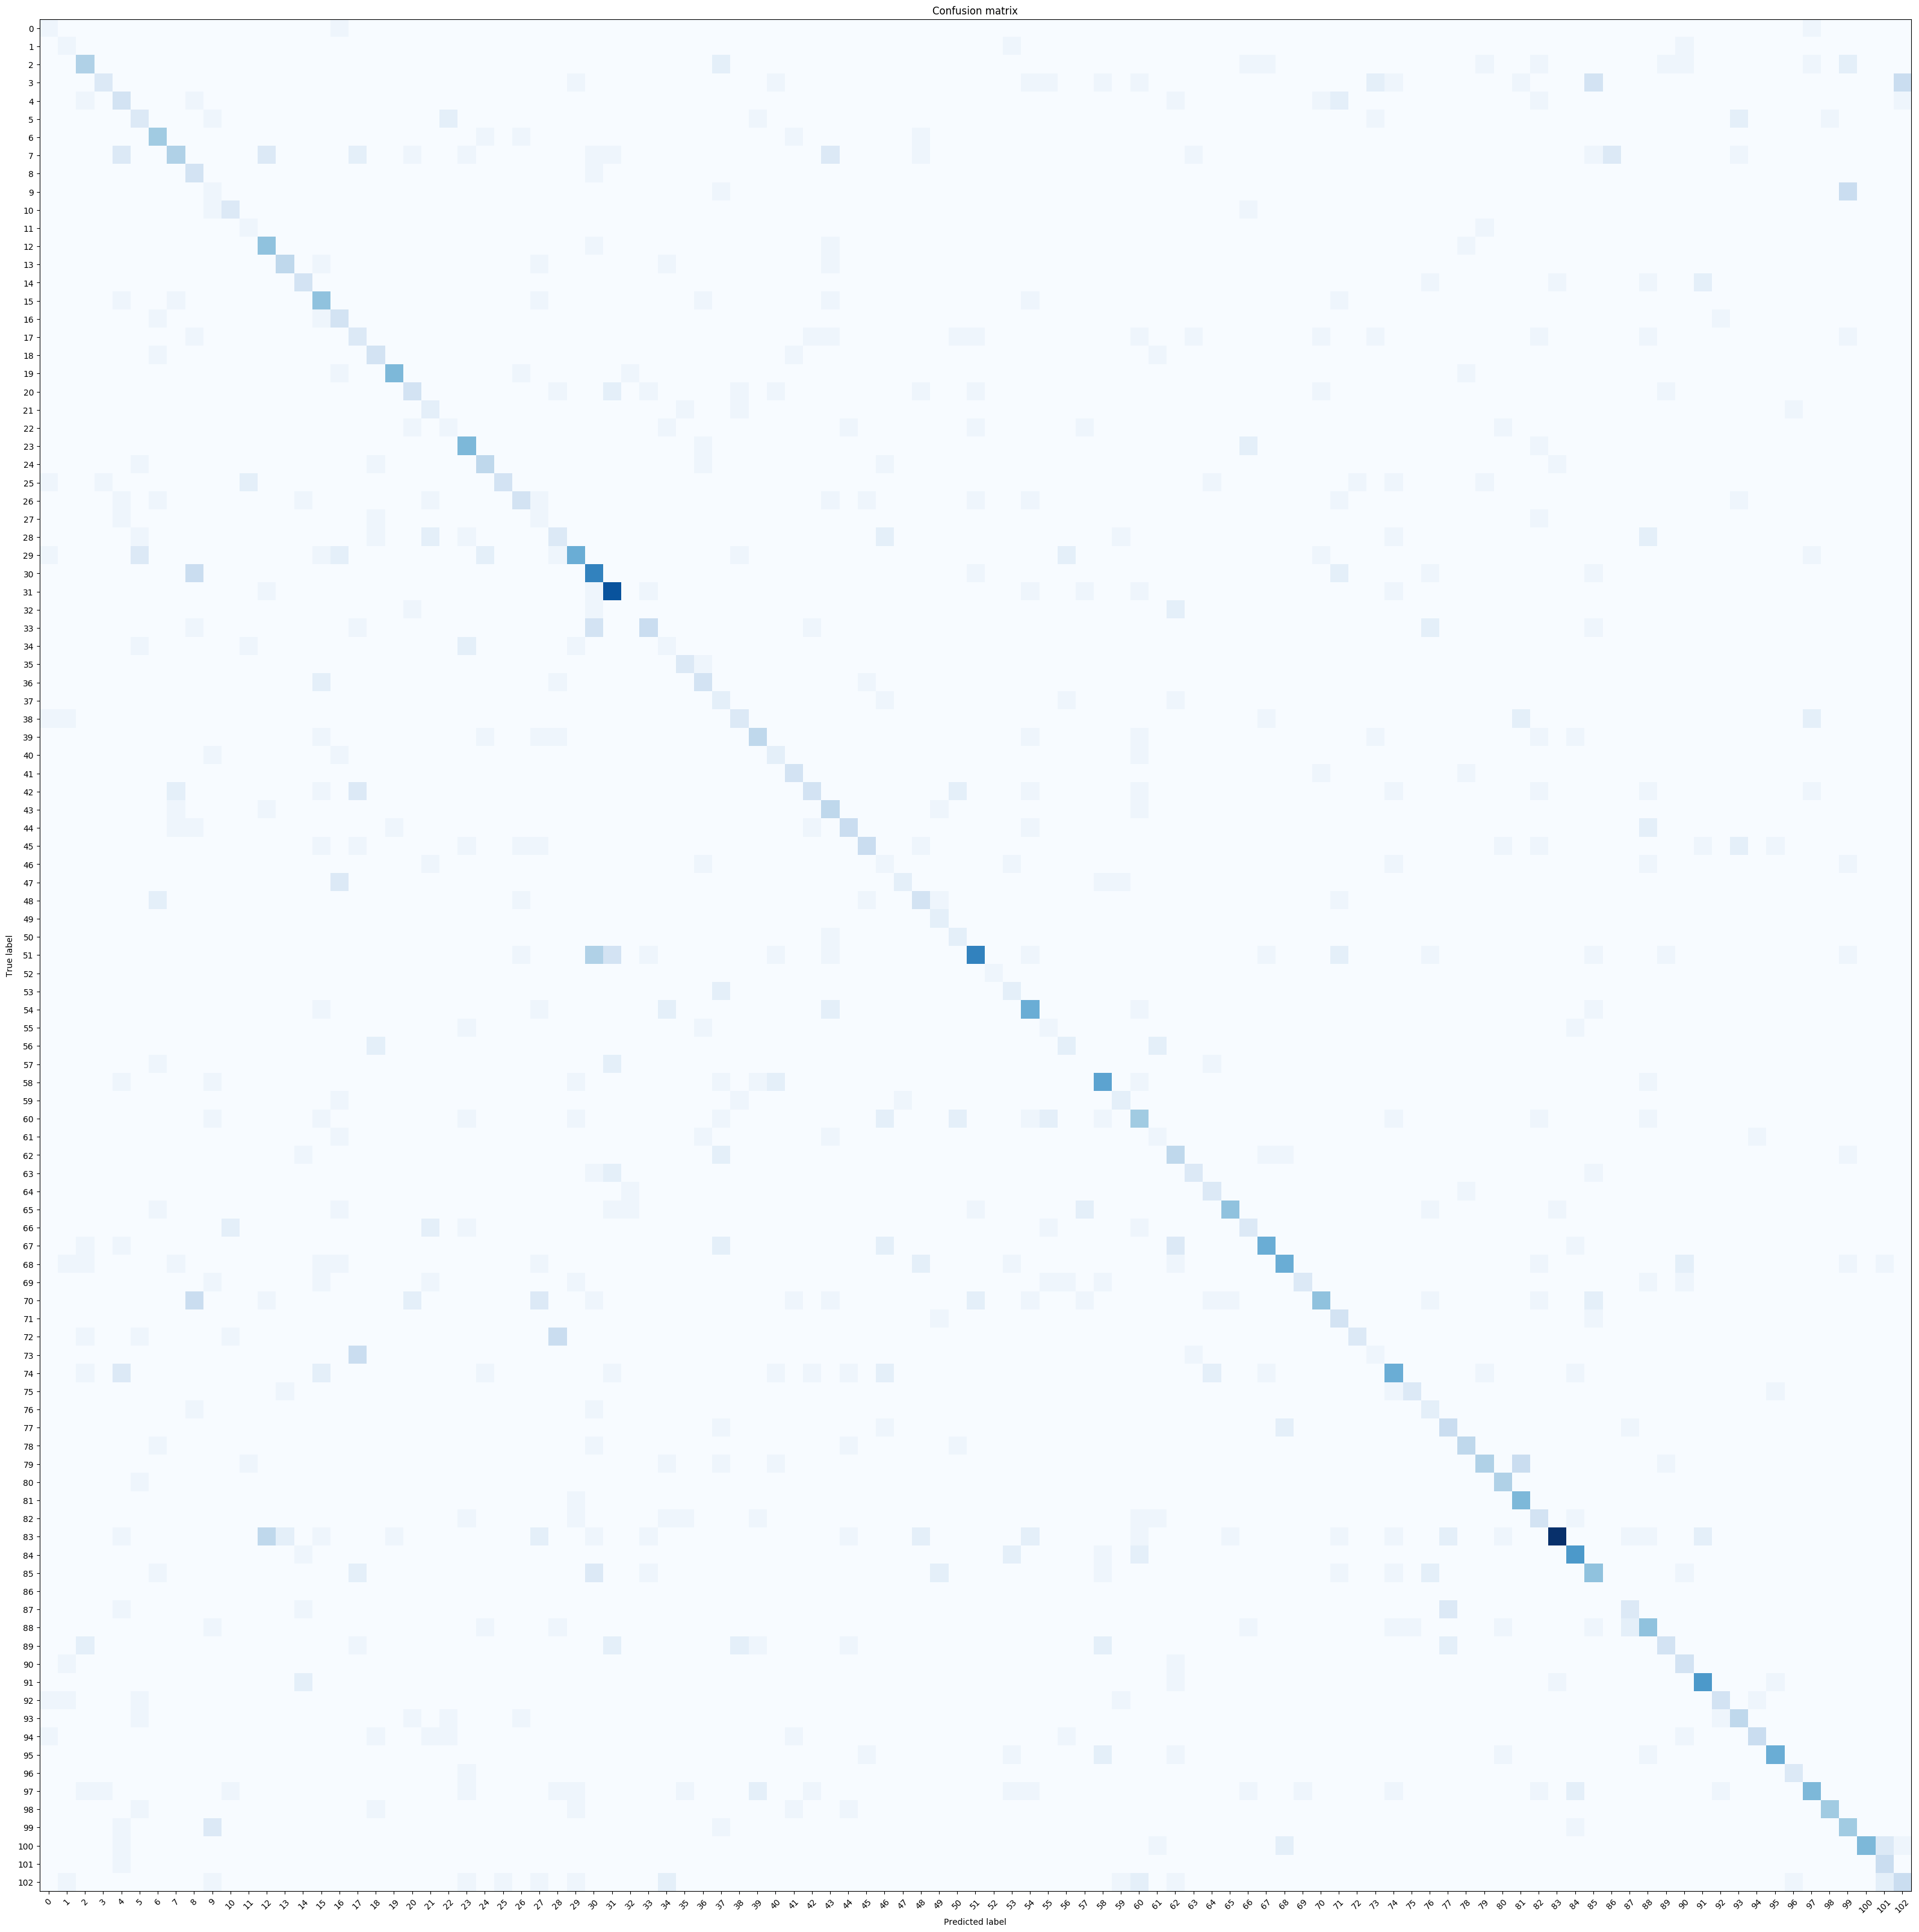
\includegraphics[width=\columnwidth]{figures/conf_mat_cnn_knn.png}
        \caption{Confusion matrix of untargeted model. x-axis corresponds to predicted label, y-axis to ground truth.}
        \label{fig:conf_mat_untargeted}
    \end{subfigure}  
    \qquad
    \begin{subfigure}[b]{0.5\columnwidth}
        \centering
        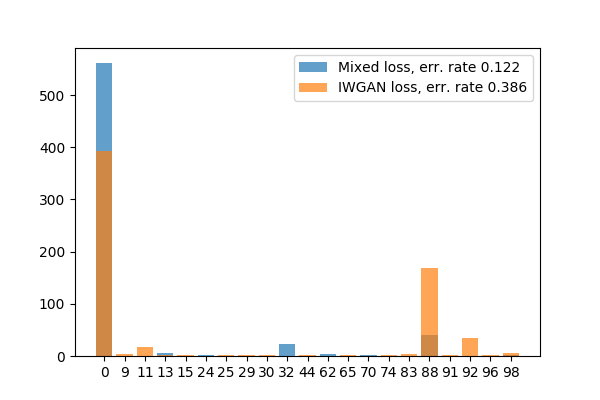
\includegraphics[width=\columnwidth]{figures/pred_comparisson_spk0.png}
        \caption{Histogram of predictions given WGAN-GP and mixed loss models. Ground truth label: 0.}
        \label{fig:pred_comp_spk0}
    \end{subfigure}
    \caption{Summary histograms of targeted attacks}
    \label{fig:confusion_matrices}
\end{figure}
